

\documentclass[a4paper,12pt]{article} % тип документа
\usepackage[margin=1in]{geometry}

% report, book

%  Русский язык

\usepackage[T2A]{fontenc}			% кодировка
\usepackage[utf8]{inputenc}			% кодировка исходного текста
\usepackage[english,russian]{babel}	% локализация и переносы
\usepackage{graphicx}                % Математика
\usepackage{amsmath,amsfonts,amssymb,amsthm,mathtools} 
\usepackage{mathtext}
\usepackage[T2A]{fontenc}
\usepackage[utf8]{inputenc}

\usepackage{wasysym}

%Заговолок
\author{Бичина Марина 
группа Б04-005 1 курса ФЭФМ}
\title{Отчет по лабораторной работе №2.1.6
Эффект Джоуля-Томсона}
\date{\today}


\begin{document} % начало документа

\maketitle
\newpage


\section{Аннотация}

\paragraph{Цель работы:}

1) определить изменения температуры углекислого газа при протекании через малопроницаемую перегородку при разных начльных значениях давления и температуры

2) вычислить по результатам опытов коэффициентов Ван-дер-Ваальса <<a>> и <<b>> \\ \\ \textbf{Оборудование:}
 
1) трубка с пористой перегородкой

2) труба Дьюара

3) термостат

4) термометры

5) дифференциальная термопара

6) микровольтрмер

7) балластный баллон

8) манометр



\section{Теоретическая часть}


Эффектом Джоуля–Томсона называется изменение температуры
газа, медленно протекающего из области высокого в область низкого давления в условиях
хорошей тепловой изоляции.
В разреженных газах,
которые приближаются по своим свойствам
к идеальному газу, при таком течении температура газа не меняется. Эффект Джоуля–Томсона демонстрирует отличие исследуемого газа от идеального.

В работе исследуется изменение температуры углекислого газа
при медленном его течении по трубке с пористой перегородкой (рисунок 1). Трубка 1 хорошо теплоизолирована.
Газ из области повышенного давления $P_1$ проходит через множество узких и длинных каналов пористой перегородки 2 в область с атмосферным давлением
$P_2$. Перепад давления $\Delta P = P_1-P_2$ из-за большого сопротивления каналов может быть заметным даже при малой скорости течения газа в трубке. Величина эффекта Джоуля–Томсона определяется по
разности температуры газа до
и после перегородки.

\subsection{Описание установки}
 
 \begin{figure}[h]

\centering

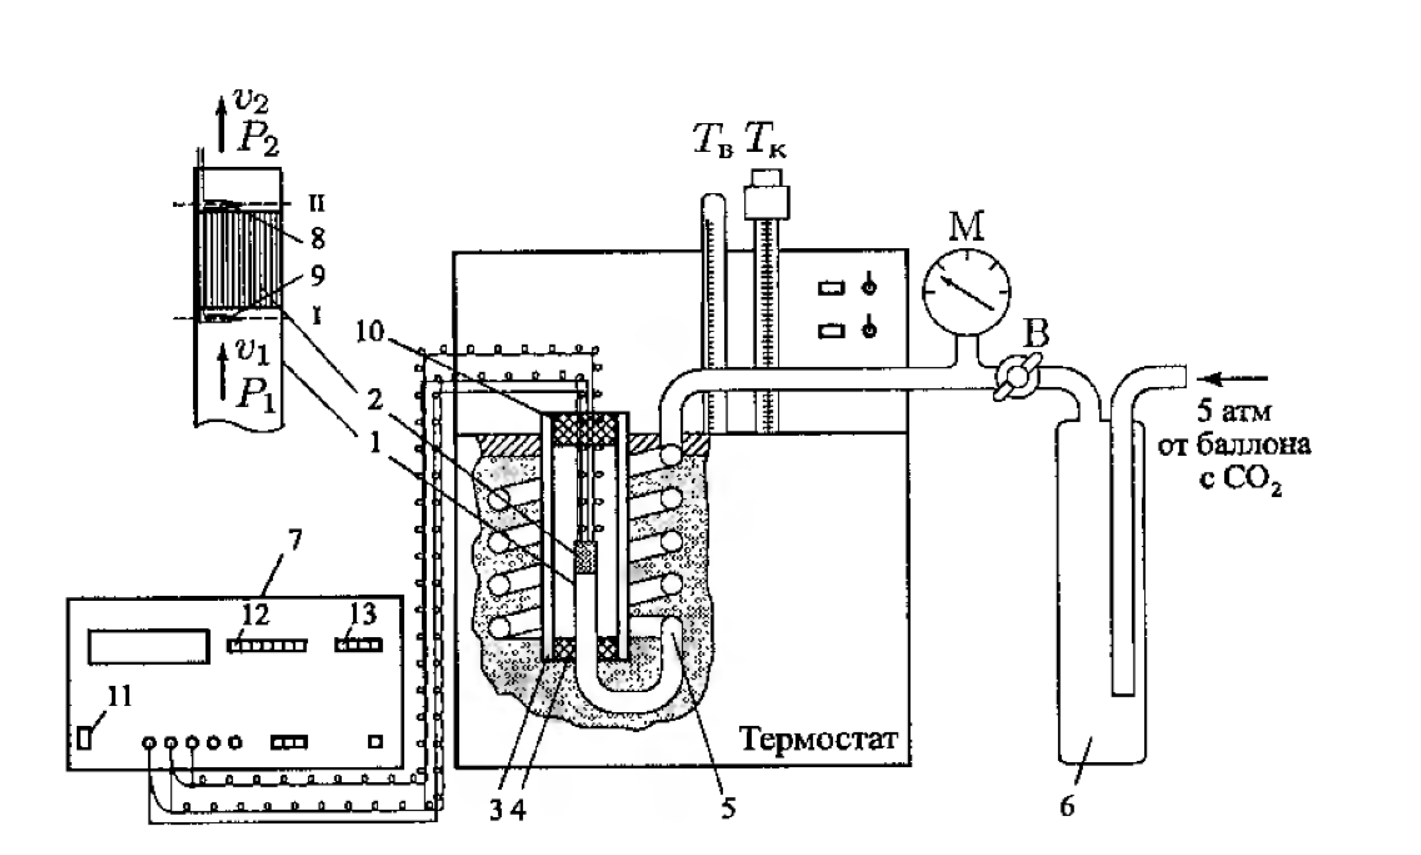
\includegraphics[width=0.8\linewidth]{lab 2.1.6.png}

\caption{Схема установки для изучения эффекта Джоуля-Томсона}

\label{fig:mpr}

\end{figure}


На схеме изображены:\\[0.1 cm]


\begin{minipage}{0.4\textwidth}
  
  1) трубка
  
  2) пористая перегородка
  
  3) трубка Дьюара
  
  4) уплотнение трубки Дьюара кольцом
  
  5) змеевик
  
  6) балластный баллон
\end{minipage}
\hfill
\begin{minipage}{0.4\textwidth}
  
  
  7) цифровой вольтметр
  
  8-9) спаи
  
  10) пробка из пенопласта
  
  11) выключатель <<Сеть>>
  
  12 кнопка <<АВП>>
  
  13 кнопка <<$U_=$>>
  
  
\end{minipage}\\[0.3 cm]


\section{Экспериментальная часть}
\subsection{Ход работы}
\begin{enumerate} 
\itemsep0em
\item Перед началом работы убедимся в том, что термостат залит водой,
а все электрические приборы заземлены.
\item Установим на контактном термометре $T_k$ температуру регулирования, близкую к комнатной, и включим термостат. 
\item Включим вольтметр. Запишим знак и величину показаний для вольтметра при $\Delta P = 0$. Используем эту величину для корректировки показаний вольтметра в дальнейших измерениях: $E = U(P)-U(0)$.

Откроем регулирующий вентиль настолько, чтобы избыточное давление составило $\Delta P \approx 4$ атм.
\item Через 10–15 минут после подачи давления запишем показания вольтметра
\item При помощи вентиля В установим давление на 0,3–0,5 атм меньше первоначального. Через 5 минут, когда
установятся давление и разность температур, вновь запишите показания манометра и вольтметра. Повторим операцию 5-7 раз для разных значениях давления при комнатной температуре.
\item Построим график зависимости $\Delta T (\Delta P)$ и по наклону определим коэффициент Джоуля-Томсона для выбраной температуры
\item Окончив измерения при комнатной температуре, установим температуру, равную $50 ^oC$. Проделаем действия, аналогичные 3-6. 
\item Проделаем измерения 3-6 для температуры $80 ^oC$
\item Произведем вычисления: найдем <<a>>, <<b>> и $T_{inv}$ для $CO_2$. Сравним их с табличными значениями
\item Обработаем результаты
\item Оценим ошибки измерений 

\end{enumerate}
\subsection{Полученные результаты}

\paragraph{Характеристики установки:}
\subparagraph{Инструментальные погрешности:}
\subparagraph{Начальные условия:}
\begin{enumerate}
\item Температура термостата: $T_0 = 18^0 C$
\item Напряжение до подачи давления: $U_0 = 0,007$ мВ
\item Давление измеряется в кгс/см$^2$, цена деления -- 0,06 кгс/см$^2$
\end{enumerate}
\begin{minipage}{0.5\textwidth}
  \begin{flushleft}

	\begin{tabular}{ | l | l | l | l |}
\hline
N & $\Delta$P,атм &T,$^0C$ & $\Delta$Т,$^0C$ \\ \hline
0 & 0.0 & 18.0 & 0.0 \\
1 & 4.065 & 18.15 & 4.322 \\
2 & 3.717 & 18.23 & 3.894 \\
3 & 3.339 & 18.29 & 3.467 \\
4 & 2.962 & 18.37 & 3.015 \\
5 & 2.671 & 18.45 & 2.663 \\
6 & 1.974 & 18.51 & 1.859 \\
7 & 1.713 & 18.62 & 1.583 \\
\hline
\end{tabular}


Таблица 1 -- данные для комнатной температуры
  \end{flushleft}
\end{minipage}
\begin{minipage}{0.5\textwidth}
  \begin{flushright}
	\begin{tabular}{ | l | l | l | l |}
\hline
N & $\Delta$P,атм &T,$^0C$ & $\Delta$Т,$^0C$ \\ \hline
0 & 0.0 & 30.06 & 0.0 \\
1 & 4.181 & 30.1 & 3.846 \\
2 & 3.862 & 30.08 & 3.462 \\
3 & 3.078 & 30.01 & 2.62 \\
4 & 2.671 & 30.02 & 2.188 \\
5 & 2.584 & 30.0 & 2.115 \\
6 & 2.236 & 30.0 & 1.755 \\
7 & 1.568 & 30.0 & 1.082 \\
\hline
\end{tabular}

 
Таблица 2 -- данные для температуры $\simeq 30$
  \end{flushright}
\end{minipage}
\end{document} % конец документа